\documentclass[11pt,a4paper]{article}
\usepackage{manuscripts/preamble/qsd_preamble}
\usepackage{orcidlink}
\usepackage{mdframed}
\usepackage[table]{xcolor}
\usepackage{tikz}
\usetikzlibrary{arrows.meta, positioning, shapes.geometric,
                fit, backgrounds, decorations.pathreplacing,
                decorations.markings}
\usepackage{booktabs}
\usepackage{array}
\geometry{margin=1in}
\hypersetup{colorlinks=true, linkcolor=blue!70!black,
  citecolor=blue!60!black, urlcolor=blue!60!black}

% --- Epistemic tags (local) -------------------------------------------------
\newcommand{\Rmark}{\textcolor{green!50!black}{\textbf{[R]}}}
\newcommand{\Cpmark}{\textcolor{blue!70!black}{\textbf{[C+]}}}
\newcommand{\Tmark}{\textcolor{orange!70!black}{\textbf{[T]}}}
\newcommand{\EXPmark}{\textcolor{red!50!black}{\textbf{[EXP]}}}

% --- Box colour palette -----------------------------------------------------
\definecolor{Rbg}{RGB}{235,255,240}
\definecolor{Rcolor}{RGB}{40,140,60}
\definecolor{Tbg}{RGB}{255,248,225}
\definecolor{Tcolor}{RGB}{160,120,20}
\definecolor{insightbg}{RGB}{255,248,225}
\definecolor{insightcol}{RGB}{160,120,20}
\definecolor{structbg}{RGB}{248,240,255}
\definecolor{structcol}{RGB}{100,40,160}
\definecolor{defbg}{RGB}{248,248,255}
\definecolor{defcol}{RGB}{40,40,120}
\definecolor{lightbg}{RGB}{245,248,255}
\definecolor{envbg}{RGB}{255,245,235}
\definecolor{envcol}{RGB}{180,100,40}
\definecolor{ctcbg}{RGB}{255,240,240}
\definecolor{ctccol}{RGB}{180,50,50}

% --- Document macros --------------------------------------------------------
\newcommand{\Cq}[4]{[\![#1,#2,#3]\!]_{#4}}
\providecommand{\Cl}[1]{\mathrm{Cl}(#1)}
\providecommand{\Hbfour}{\mathrm{Hb}_4}
\newcommand{\Op}{\mathcal{O}}
\newcommand{\Env}{\mathcal{E}}
\newcommand{\proj}[1]{\Pi_{#1}}
\newcommand{\Ms}{M_{\mathbf{s}}}

%==============================================================================
\title{
  \textbf{The Observer}\\[0.5em] 
  \Large A Formal Definition from Quantum Error Correction\\[0.8em]
  \large QSD Phase 2 --- Part I, Supplement S9
}
\author{Marek Hubka\, \orcidlink{0009-0003-2476-9017}
  \thanks{Independent Researcher, Czech Republic.\; \\
    \href{mailto:marek@tidesofuncertainty.com}{marek@tidesofuncertainty.com}.}}
\date{\today}

\begin{document}
\maketitle

%==============================================================================
\begin{abstract}
\noindent
Part~I \S8 defines an observer as an $[\![n,1,d]\!]_q$ system performing syndrome measurements on its environment, with the $q=2$ ground-state observer the unique thermodynamically stable realisation. This supplement provides the complete derivation.

We show that the QECC structure of an observer is not postulated. It follows from two functional requirements: stable record-keeping under environmental perturbation motivates error-correction ($d\geq3$), and definite measurement outcomes motivate one logical record qubit ($k=1$) --- with the algebraic force supplied by the CTC-freedom argument of Supplement~S8 (triple equivalence theorem). Thermodynamic stability against unbounded entropy accumulation under the observer's own correction cycles forces $q=2$ via Landauer's principle, exactly the argument applied to the universe's code in P1 \S5. Finally, the Heisenberg cut is derived from the syndrome-measurement structure, and measurement is identified with syndrome extraction: given the standard quantum formalism, the Born weights and the L\"uders update apply to it as to any projective measurement. The Born rule itself is \emph{used, not derived} --- a derivation would require independent premises (e.g.\ Gleason-type noncontextuality across all contexts) that code structure does not supply --- and outcome selection, the measurement problem proper, is explicitly out of scope.
\end{abstract}

\begin{mdframed}[backgroundcolor=insightbg,linecolor=insightcol,
  linewidth=1.5pt, skipabove=8pt, skipbelow=8pt]
\textbf{Supplement context.}\quad
This document is Supplement~S9 of Part~I~\cite{Hubka2026QSD}. Part~I \S8 states the observer definition as~\Rmark; this supplement provides the complete derivation. The $k=1$ argument (\S\ref{sec:k1}) uses the triple equivalence proved in Supplement~S8~\cite{Hubka2026QSDSupp}. Results established here may be cited as ``Supplement~S9''~\cite{Hubka2026QSDSupp}.
\end{mdframed}

\newpage
\tableofcontents
\newpage

%==============================================================================
\section{What an Observer Must Do}
\label{sec:what_obs}
%==============================================================================

We derive the QECC structure of an observer from two functional requirements, with no postulate added.

An observer is a physical system that performs measurements on its environment and retains stable records of those measurements --- the physical-system reading of the observer that runs from von Neumann's measurement chain~\cite{vNeumannQM} through Wigner~\cite{Wigner1961} to decoherence theory~\cite{Zurek2003}. Each requirement has a direct code-theoretic translation.

\paragraph{Stable records require error correction.}
Any physical memory register is subject to environmental perturbation: thermal noise, decoherence, single-qudit Pauli errors. A record that degrades under perturbation is not a record --- the stability of records under environmental monitoring is precisely what einselection~\cite{Zurek2003} and quantum Darwinism~\cite{Zurek2009} identify as the mark of the classical. For a memory register to maintain stable logical states under every single-qudit error, it must be capable of \emph{correcting} those errors --- not merely detecting them. The detection-only case ($d=2$) tells the observer that its memory has been corrupted but cannot recover the original content, leaving every measurement unrepeatable. The protected case requires
\begin{equation}
  d \;\geq\; 3,
  \label{eq:d3_obs}
\end{equation}
the same constraint derived for the universe's code in P1 \S3.1~\cite{Hubka2026QSD}, here applied to the observer subsystem; that stable quantum memory requires active error correction is the founding observation of the field~\cite{Shor1995,Steane1996}.

\paragraph{Definite outcomes require a protected record register ($k=1$).}
Each act of measurement must terminate in a definite, stable record --- an outcome (``$+$'' or ``$-$'', ``error in sector $s$'' or ``no error''), not a coherent superposition of outcomes. Holding a committed record requires a protected register, and the minimal such register is one logical qubit, which commits at most one classical bit per write:
\begin{equation}
  k \;=\; 1.
  \label{eq:k1_obs}
\end{equation}
This operational reading \emph{motivates} $k=1$; the argument that carries the weight --- why $k\geq2$ actively fails --- is algebraic and follows in \S\ref{sec:k1}. (What the record can and cannot hold relative to the four-bit syndrome is made precise in \S\ref{sec:measurement}.)

\paragraph{Therefore.}
An observer performing measurements and retaining their results is a $[\![n,1,d]\!]_q$ stabiliser system --- a quantum error-correcting code --- with $d\geq3$ for memory stability and $k=1$ per measurement event. The QECC structure is not assumed. It follows from what observation \emph{is}: the production and storage of classical records under environmental perturbation.

\begin{mdframed}[backgroundcolor=defbg,linecolor=defcol,linewidth=1.5pt]
\textbf{Observer as QECC (definition).}\quad
An observer is a physical system performing syndrome measurements on its environment and retaining the results in a $[\![n,1,d]\!]_q$ logical register. The QECC structure is not postulated --- it is motivated by stable memory ($d\geq3$) and definite outcomes ($k=1$), constraint arguments tagged~\Cpmark\ with premises stated in \S\ref{sec:d3}--\S\ref{sec:k1}. The $q=2$ observer is the unique thermodynamically stable ground state~\Tmark\ ($\Sigma=1$).
\end{mdframed}

%==============================================================================
\section{The $d\geq3$ Constraint for Observer Memory}
\label{sec:d3}
%==============================================================================

We make the $d\geq3$ requirement of \S\ref{sec:what_obs} precise.
\emph{Premise of this section~\Cpmark: the observer's record is itself a
quantum register whose dominant noise channel is single-qudit Pauli
errors --- the same noise model under which the universe's code is selected
in P1 \S3.1.}

An observer's memory register stores committed measurement outcomes. Each stored outcome is, after extraction from the environment, a classical bit. Single-qudit Pauli errors on the memory's physical register are the dominant noise channel:
\begin{itemize}\setlength\itemsep{2pt}
  \item $d=1$: any single environmental perturbation corrupts the record irreversibly. The observer cannot trust its own memory; no stable physical inference is possible.
  \item $d=2$: the observer can detect that its memory has been corrupted but cannot recover the original record. Every measurement is unrepeatable: the observer cannot verify that two queries of the same record produced consistent answers.
  \item $d\geq3$: the syndrome uniquely identifies the single-qudit error and the correction operator is well-defined. The record survives.
\end{itemize}

The argument is structurally identical to P1 \S3.1, now read as a constraint on the observer subsystem rather than the universe's code as a whole. The same physical principle --- that single-qudit errors must be correctable, not merely detectable --- applies whenever a stabiliser code is required to maintain a stable logical state.

\begin{mdframed}[backgroundcolor=Rbg,linecolor=Rcolor,linewidth=1.5pt]
\textbf{Observer memory constraint\,\Cpmark.}\quad
\emph{Premise: records are quantum registers under single-qudit Pauli noise.} Then an observer's memory register requires $d\geq3$ for stable record-keeping --- the same error-correction constraint derived for the universe's code in Part~I, \S3.1~\cite{Hubka2026QSD}, applied to the observer as a physical subsystem.
\end{mdframed}

%==============================================================================
\section{The $k=1$ Constraint: CTC-Free Observer Memory}
\label{sec:k1}
%==============================================================================

We make the $k=1$ requirement of \S\ref{sec:what_obs} precise via the triple equivalence theorem of Supplement~S8.

\paragraph{Why $k\geq2$ fails for an observer.}
Suppose an observer has $k\geq2$ logical qubits in its memory register, intended to record outcomes of two or more sequential measurements simultaneously. Then the apparent code carries crossing operators between its own logical qubits. Concretely, with $k=2$ and outcomes $m_1$ and $m_2$ stored in the two logical qubits, the simplest crossing operator is $C_{12}=\bar X_1\bar X_2$. Its action on the joint logical record is the channel
\begin{equation}
  \Ms(\rho_L)
  \;=\; (\bar X_1\otimes\bar X_2)\,(\rho_1\otimes\rho_2)\,
        (\bar X_1\otimes\bar X_2)^\dagger
  \;=\; (X\rho_1 X)\otimes(X\rho_2 X),
\end{equation}
which has Deutsch fixed point $\rho^*=I/4$ (Supplement~S8, \S2~\cite{Hubka2026QSDSupp}). The two records both equilibrate to maximally mixed marginals and become information-free. The observer cannot subsequently distinguish which measurement produced which outcome --- its records are self-contradictory internal CTCs.

\paragraph{The triple equivalence applied.}
Supplement~S8's triple equivalence theorem states that for any stabiliser code with $n=5$, $d=3$, the three conditions
\[
  \binom{k}{2}\geq 1
  \;\Longleftrightarrow\;
  \text{Deutsch-CTC channel exists}
  \;\Longleftrightarrow\;
  \mathcal{I}^2=+1
\]
are mutually equivalent and absent simultaneously only at $k=1$~\cite{Hubka2026QSDSupp}. Applied to the observer subsystem, this rules out $k\geq2$ on three independent grounds: a $k\geq2$ observer would carry crossing pairs between its own logical qubits, would equilibrate its joint record to $I/2^k$ under any internal correction cycle, and would lack a canonical complex structure for the dynamics that update the record.

\paragraph{$k=1$ uniquely sufficient.}
At $k=1$ there are zero crossing pairs ($\binom{1}{2}=0$), no Deutsch-CTC channel arises, and $\mathcal{I}^2=-1$ in the syndrome algebra $\Cl{1,n-2}$. The record is causally consistent and supports unitary evolution conditioned on classical syndrome outcomes. Each write commits at most one classical bit to the record (\S\ref{sec:measurement}).

\begin{mdframed}[backgroundcolor=Rbg,linecolor=Rcolor,linewidth=1.5pt]
\textbf{Observer $k=1$ constraint\,\Cpmark.}\quad
\emph{Premise: the crossing channels admitted by a $k\geq2$ register are dynamically realised under the observer's own correction cycles.} Then $k\geq2$ observer memory equilibrates its joint record to the maximally mixed $\rho^*=I/2^k$ --- internal CTCs in the observer's own memory --- and $k=1$ is uniquely consistent. The underlying triple equivalence ($\binom{k}{2}\geq1 \Leftrightarrow$ Deutsch channel $\Leftrightarrow \mathcal{I}^2=+1$) is algebra and remains~\Rmark: Supplement~S8~\cite{Hubka2026QSDSupp}.
\end{mdframed}

%==============================================================================
\section{The $q=2$ Constraint: Thermodynamically Stable Observer}
\label{sec:q2}
%==============================================================================

\paragraph{Empirical basis.}
The Second Law of Thermodynamics and Landauer's principle are not axioms of QSD. They are empirically established laws of physics: the minimum energy cost to erase one bit of classical information is $k_B T\ln 2$, derived theoretically by Landauer~\cite{Landauer1961} and verified experimentally in colloidal-particle double-well experiments to within $5\%$~\cite{Berut2012}; for the general thermodynamics of computation see~\cite{Bennett1982}. Part~I \S5~\cite{Hubka2026QSD} develops the empirical basis in detail and uses it to select the $q=2$ ground state for the universe's code. This supplement applies the same argument to the observer: an observer is itself a physical system running error-correction cycles, and Landauer's bound binds it just as firmly as it binds the rest of the lattice. The epistemic tag~\Tmark\ records this status --- a mandatory consistency condition with empirically established thermodynamics, not a framework-internal conjecture.

\paragraph{The observer's own filling fraction.}
Each syndrome-measurement cycle that the observer performs on its own memory register erases the prior outcome and records a new one. Every erasure dissipates at minimum $k_BT\ln 2$ per syndrome bit measured. The relevant figure of merit is the syndrome filling fraction of the observer's code,
\begin{equation}
  \Sigma(q) \;=\; \frac{1+5(q^2-1)}{q^4} \;=\; \frac{5q^2-4}{q^4},
  \label{eq:sigma_obs}
\end{equation}
identical in form to the lattice expression of P1 \S5.2 because the observer is itself a $[\![5,1,3]\!]_q$ code block. For $q=2$: $\Sigma=1$ exactly --- every syndrome slot corresponds to a correctable error, no syndrome bit is wasted, and the observer's correction cycle dissipates only the minimum mandatory $k_BT\ln 2$ per genuine erasure. For all $q\geq3$: $\Sigma<1$, so a fraction $1-\Sigma$ of every cycle is dissipated against \emph{ghost} syndrome slots that contain no correctable error. This excess dissipation accumulates without bound over the observer's operational lifetime.

\paragraph{Stability requires $\Sigma=1$.}
A thermodynamically stable observer --- one whose entropy production per cycle saturates the Landauer minimum and does not accumulate irreducible overhead --- requires $\Sigma=1$. By the same factorisation $(q^2-1)(q^2-4)=0$ that selected the universe's alphabet (P1 \S3.5), this is achieved uniquely at $q=2$. All $q\geq3$ observers are thermodynamically excited states relative to the $q=2$ ground state, with overhead scaling as $q^{-2}$.

\paragraph{Status.}
This is~\Tmark, not an additional QSD assumption about observers and not a conjecture: a $q\geq3$ observer would violate the Second Law in the operational sense that its accumulated irreducible entropy would diverge with operation time. The $q=2$ observer is therefore not chosen among equally valid alternatives; it is the unique thermodynamically stable realisation of an observer in any thermal environment.

\newpage

\begin{mdframed}[backgroundcolor=Tbg,linecolor=Tcolor,linewidth=1.8pt]
\textbf{Thermodynamically stable observer\,\Tmark.}\quad
The Second Law and Landauer's principle (Part~I \S5~\cite{Hubka2026QSD}, both empirically established) require $\Sigma(q)=1$ for an observer that does not accumulate unbounded entropy. This is satisfied uniquely at $q=2$. All $q\geq3$ observers carry irreducible thermodynamic overhead per correction cycle and are thermodynamically excited states. The $q=2$ observer is the unique ground-state observer.
\end{mdframed}

%==============================================================================
\section{Measurement as Syndrome Extraction}
\label{sec:measurement}
%==============================================================================

We now identify measurement with syndrome extraction and establish exactly what that identification delivers. Given the standard quantum formalism, syndrome extraction is a projective measurement, so the Born weights and the L\"uders update apply to it as to any other; the identification fixes the outcome alphabet, the repeatability of records, and (in \S\ref{sec:cut}) the Heisenberg cut. What it does \emph{not} do is derive the Born rule from code structure, or resolve which outcome obtains; the epistemic accounting is stated explicitly below.

\paragraph{Setup.}
The observer's code consists of $n-k=4$ stabiliser generators $S_1,\ldots,S_4$ acting on a five-qubit code block, with one logical qubit reserved for the record. To measure, the observer performs the four stabiliser measurements on a \emph{neighbouring} five-qubit block --- the environment block; its own registers are not the target (\S\ref{sec:cut}). Each generator yields one classical bit; the four-bit string $s=(s_1,s_2,s_3,s_4)\in\{0,1\}^4$ is the syndrome outcome and parametrises the $2^4=16$ orthogonal syndrome subspaces of the environment block's Hilbert space.

\paragraph{Born weights on syndrome sectors (given the standard formalism).}
Let $\proj{s}$ denote the orthogonal projector onto the syndrome-$s$ subspace. Given that states are density operators and outcomes label orthogonal projectors --- the standard formalism --- the probability of syndrome $s$ is
\begin{equation}
  p_s \;=\; \mathrm{tr}\!\left(\proj{s}\,\rho_E\,\proj{s}^\dagger\right)
  \;=\; \mathrm{tr}\!\left(\proj{s}\,\rho_E\right).
  \label{eq:born}
\end{equation}
This is the Born rule~\cite{Born1926} \emph{applied to} syndrome extraction, and it is used here, not derived: the trace form is part of the formalism the code inhabits. A derivation would require independent premises --- for instance Gleason-type noncontextual additivity across \emph{all} measurement contexts~\cite{Gleason1957}, which the finite context family of a code block does not supply (on any single decomposition, every probability assignment over the sixteen sectors is realised by some state); on the $k=1$ record space, of dimension two, Gleason's theorem is inapplicable in principle (the POVM extension~\cite{Busch2003} does reach dimension two, but only by assuming additivity over the full effect algebra --- a strictly stronger premise than the code's projective structure supplies). Within the code's native stabiliser states every $p_s$ is $0$ or $2^{-j}$; continuous weights enter only through the measured state itself.

\paragraph{Post-measurement update.}
After the observer reads syndrome $s$, the environment block's state is the conditional state:
\begin{equation}
  \rho_E \;\longmapsto\;
  \rho_E^{(s)}
  \;=\; \frac{\proj{s}\,\rho_E\,\proj{s}^\dagger}{p_s}.
  \label{eq:update}
\end{equation}
This is the L\"uders update~\cite{Lueders1951}, the standard post-measurement rule; read as conditioning on the recorded outcome it is the quantum counterpart of Bayesian updating~\cite{Bub1977} (its uniqueness among instruments follows from repeatability and minimal disturbance --- premises, if one insists on deriving it). Which outcome obtains --- the selection itself --- is not addressed by this supplement: the identification of measurement with syndrome extraction is compatible with the standard interpretive options and decides among none of them.

\paragraph{The logical qubit as record: the information budget.}
Each syndrome-extraction cycle produces a classical four-bit string $s$ --- \emph{transient working data}. All four bits are required to select the correction: by the perfect-code property $2^4 = 1 + 3\cdot5$, every nontrivial syndrome names exactly one single-qubit error. After use, the register holding $s$ is erased, at the Landauer minimum of $4\,k_BT\ln2$ per cycle (\S\ref{sec:q2}) --- in code units, $4\ln2 = 1/\Hbfour$, the reciprocal of the holographic bit density. The $k=1$ logical qubit is the observer's protected record \emph{slot}: per write it commits at most one classical bit --- a chosen summary $f(s)$ (in the minimal reading, ``error seen / not seen'') --- never the string $s$ itself, since no injective map from sixteen syndromes into a two-state record exists. The framework's persistent records live elsewhere: the classical bit written at the snap, and the frozen ledger's two-bit forensic capacity. The four stabiliser generators of $\Cq{5}{1}{3}{2}$, written explicitly,
\begin{equation}
  S_1 = XZZXI,\quad S_2 = IXZZX,\quad
  S_3 = XIXZZ,\quad S_4 = ZXIXZ,
  \label{eq:stabs}
\end{equation}
fix the sixteen-sector decomposition; for a definite single-qubit Pauli error the outcome is deterministic and identifies the error uniquely.

\begin{figure}[h]
\centering
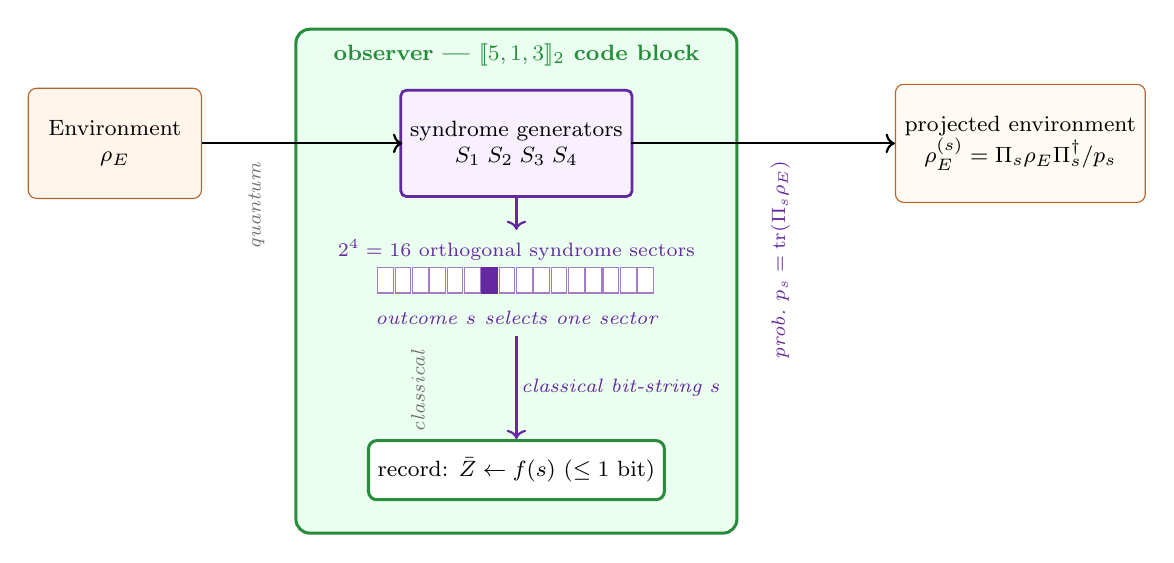
\begin{tikzpicture}[every node/.style={font=\footnotesize}]

% ---- environment (input) ----
\node[draw=envcol, fill=envbg, rounded corners=3pt, minimum width=2.2cm,
      minimum height=1.4cm, align=center] (env) at (0.7,1.6)
      {Environment\\$\rho_E$};

% ---- the observer container ----
\draw[draw=Rcolor, fill=Rbg, line width=1.1pt, rounded corners=5pt]
     (3.0,-3.35) rectangle (8.6,3.05);
\node[Rcolor, font=\footnotesize\bfseries] at (5.8,2.72)
     {observer --- $\Cq{5}{1}{3}{2}$ code block};

% generators
\node[draw=structcol, fill=structbg, rounded corners=2pt, line width=1pt,
      minimum width=2.9cm, minimum height=1.35cm, align=center]
      (synd) at (5.8,1.6)
      {syndrome generators\\$S_1\;S_2\;S_3\;S_4$};

% 16-sector strip (one sector selected)
\node[structcol, font=\scriptsize] at (5.8,0.25)
     {$2^4 = 16$ orthogonal syndrome sectors};
\foreach \i in {0,...,15} {
  \pgfmathsetmacro{\xx}{4.04 + \i*0.22}
  \ifnum\i=6
    \draw[fill=structcol, draw=structcol] (\xx,-0.30) rectangle (\xx+0.20,0.02);
  \else
    \draw[fill=white, draw=structcol!60] (\xx,-0.30) rectangle (\xx+0.20,0.02);
  \fi
}
\node[structcol, font=\scriptsize\itshape] at (5.8,-0.62)
     {outcome $s$ selects one sector};

% record
\node[draw=Rcolor, fill=white, rounded corners=3pt, line width=1.1pt,
      minimum width=3.0cm, minimum height=0.75cm, align=center]
      (rec) at (5.8,-2.55)
      {record: $\bar Z \leftarrow f(s)$ ($\leq 1$ bit)};

% ---- projected environment (output) ----
\node[draw=envcol, fill=envbg!55, rounded corners=3pt, minimum width=3.1cm,
      minimum height=1.5cm, align=center] (envout) at (12.2,1.6)
      {projected environment\\$\rho_E^{(s)} = \proj{s}\rho_E\proj{s}^{\dagger}/p_s$};

% ---- quantum rail ----
\draw[->, thick] (env.east) -- (4.35,1.6);
\draw[->, thick] (7.25,1.6) -- (envout.west);
\node[structcol, font=\scriptsize\itshape, rotate=90] at (9.15,0.12)
     {prob.\ $p_s=\mathrm{tr}(\proj{s}\rho_E)$};
\node[black!55, font=\scriptsize\itshape, rotate=90] at (2.5,0.8) {quantum};

% ---- classical drop ----
\draw[->, thick, structcol] (synd.south) -- (5.8,0.5);
\draw[->, thick, structcol] (5.8,-0.85) -- (rec.north)
     node[midway, right=-2pt, font=\scriptsize\itshape]
     {classical bit-string $s$};
\node[black!55, font=\scriptsize\itshape, rotate=90] at (4.55,-1.55)
     {classical};

\end{tikzpicture}
\caption{Measurement as syndrome extraction. The environment block enters
the observer's measurement; the four generators project it onto one of
$2^4=16$ orthogonal syndrome sectors (strip; the selected sector shown
filled). The quantum branch (horizontal) carries the projected state
$\rho_E^{(s)}=\proj{s}\rho_E\proj{s}^{\dagger}/p_s$ with Born weight
$p_s=\mathrm{tr}(\proj{s}\rho_E)$ --- the Born rule \emph{applied} to
syndrome extraction, given the standard formalism. The classical branch
(vertical) carries the outcome string $s$ to the correction step; the
record commits at most a one-bit summary $f(s)$, while $s$ itself is
consumed and erased at $4\ln2 = 1/\Hbfour$ per cycle (\S\ref{sec:q2}).}
\label{fig:measurement}
\end{figure}

\begin{mdframed}[backgroundcolor=Rbg,linecolor=Rcolor,linewidth=1.5pt]
\textbf{Measurement = syndrome extraction.}\quad
\sloppy The identification is structural\,\Rmark: outcomes are the sixteen syndrome sectors, records are logical-qubit writes, and repeated measurements agree. \emph{Given} the standard quantum formalism, the Born weights $p_s = \mathrm{tr}(\proj{s}\,\rho_E)$ and the L\"uders update $\rho_E\mapsto\proj{s}\rho_E\proj{s}^\dagger/p_s$ apply to syndrome extraction as to any projective measurement (\Rmark\ given QM). The Born rule itself is imported from that formalism, not derived from the code; outcome selection is out of scope.
\end{mdframed}

%==============================================================================
\section{The Observer-Environment Split}
\label{sec:split}
%==============================================================================

The split between observer and environment is the split between the syndrome-measuring subsystem (the observer's $[\![n,1,d]\!]_2$ code block) and the physical qubits the observer measures (the environment). The split is not added to the formalism; it is the natural boundary defined by which qubits are inside the observer's stabiliser group and which are outside.

\paragraph{Anchor-dependence and gauge.}
A given physical configuration admits more than one valid observer-environment split. The observer's anchor qubit (the qubit aligned with the time direction at a given tick --- see Part~II~\cite{Hubka2026QSD}) selects one of the five $C_5$ vertices as the privileged time direction; permuting the anchor through the $C_5$ orbit cycles through five different splittings of the same five-qubit register into ``observer'' and ``environment'' roles. More generally, the four spatial vertices form the $K_4$ subgraph whose automorphism group is $S_4$; permuting these vertices is a gauge transformation of the observer-environment split.

\paragraph{Predictions are gauge-invariant.}
All physical predictions are invariant under the $S_4$ action on the $K_4$ vertices: syndrome probabilities $p_s$, the projected environment state $\rho_E^{(s)}$, and the record updates of the logical qubit are unchanged when the anchor is rotated through the $C_5$ orbit and the spacelike vertices are permuted. In coordinate-free language, the Born rule and the post-measurement update of \S\ref{sec:measurement} depend only on the projector structure $\{\proj{s}\}$ as a partition of the environment Hilbert space, which is itself preserved by the $S_4$ gauge. The split is a coordinate choice; the physics is not.

\paragraph{Consequence.}
Different observers in the lattice --- differing by anchor and by which $K_4$ vertex they identify with the time direction --- perform different syndrome decompositions of the same environmental state, but agree on every syndrome probability and every correction decision. This is the formal version of the statement that ``different observers see the same physics in different coordinates'' --- the code-theoretic counterpart of the relational reading of quantum states~\cite{Rovelli1996,Everett1957}.

\begin{figure}[h]
\centering
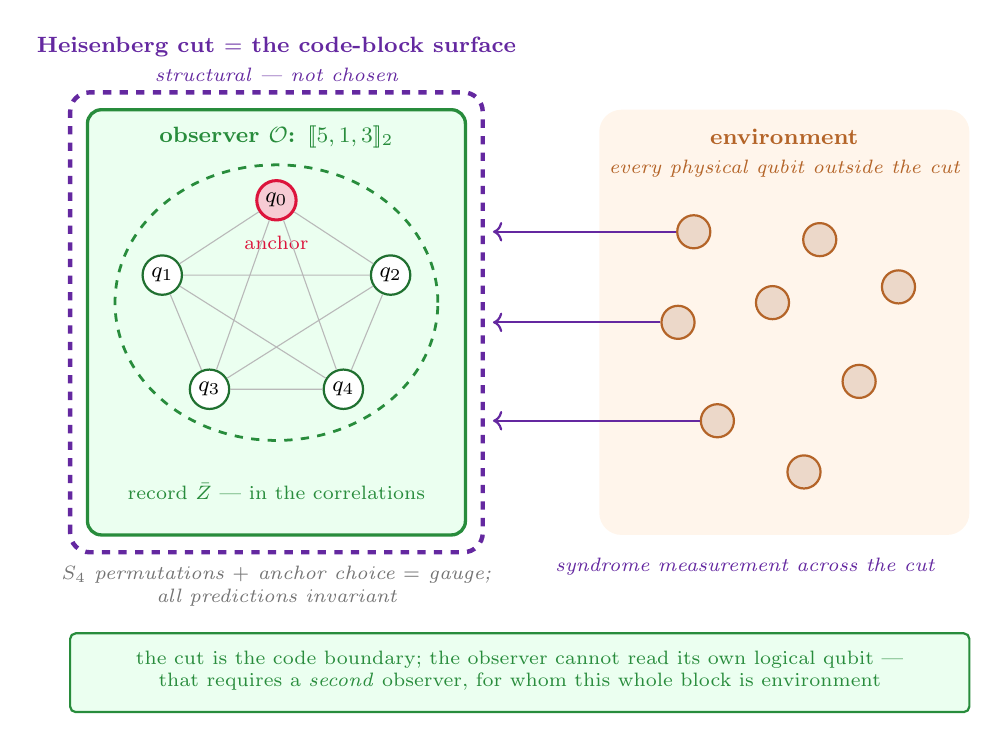
\begin{tikzpicture}[
  every node/.style={font=\footnotesize},
  qbit/.style={circle, draw=Rcolor!80!black, fill=white, line width=0.8pt,
               minimum size=0.5cm, inner sep=0pt},
  envq/.style={circle, draw=envcol, fill=envcol!25, line width=0.8pt,
               minimum size=0.42cm, inner sep=0pt}
]
\definecolor{anchorcolor}{RGB}{220,20,60}

% ---- the Heisenberg cut = the code-block surface ----
\draw[structcol, ultra thick, dashed, rounded corners=7pt]
     (-2.62,-2.92) rectangle (2.62,2.92);
\node[structcol, font=\footnotesize\bfseries, align=center] at (0,3.5)
     {Heisenberg cut $=$ the code-block surface};
\node[structcol, font=\scriptsize\itshape] at (0,3.14)
     {structural --- not chosen};

% ---- observer block ----
\draw[draw=Rcolor, fill=Rbg, line width=1.2pt, rounded corners=5pt]
     (-2.4,-2.7) rectangle (2.4,2.7);
\node[Rcolor, font=\footnotesize\bfseries] at (0,2.35)
     {observer $\mathcal{O}$: $\Cq{5}{1}{3}{2}$};

% K5 graph; anchor marked
\node[qbit, fill=anchorcolor!22, draw=anchorcolor, line width=1.1pt]
     (q0) at (0,1.55) {$q_0$};
\node[anchorcolor, font=\scriptsize, anchor=south, align=center] at (0.0,0.8) {anchor};
\node[qbit] (q1) at (-1.45,0.6) {$q_1$};
\node[qbit] (q4) at ( 1.45,0.6) {$q_2$};
\node[qbit] (q2) at (-0.85,-0.85) {$q_3$};
\node[qbit] (q3) at ( 0.85,-0.85) {$q_4$};
\draw[gray!55] (q0)--(q1) (q0)--(q2) (q0)--(q3) (q0)--(q4)
               (q1)--(q2) (q1)--(q3) (q1)--(q4)
               (q2)--(q3) (q2)--(q4) (q3)--(q4);

% the k=1 record: in the correlations, not a sixth qubit
\draw[Rcolor, dashed, line width=1pt] (0,0.25) ellipse (2.05 and 1.75);
\node[Rcolor, font=\scriptsize] at (0,-2.15)
     {record $\bar Z$ --- in the correlations};

% S4 gauge note
\node[black!55, font=\scriptsize\itshape, align=center] at (0,-3.35)
     {$S_4$ permutations $+$ anchor choice $=$ gauge;\\
      all predictions invariant};

% ---- environment: no box -- only the cut is a boundary ----
\fill[envbg, rounded corners=8pt] (4.1,-2.7) rectangle (8.8,2.7);
\node[envcol, font=\footnotesize\bfseries] at (6.45,2.35) {environment};
\node[envcol, font=\scriptsize\itshape] at (6.45,1.95)
     {every physical qubit outside the cut};
\node[envq] (e1) at (5.3,1.15) {};
\node[envq] (e2) at (6.9,1.05) {};
\node[envq] (e3) at (7.9,0.45) {};
\node[envq] (e4) at (5.1,0.0) {};
\node[envq] (e5) at (6.3,0.25) {};
\node[envq] (e6) at (7.4,-0.75) {};
\node[envq] (e7) at (5.6,-1.25) {};
\node[envq] (e8) at (6.7,-1.9) {};

% ---- syndrome measurement across the cut ----
\draw[->, thick, structcol] (e1.west) -- (2.75,1.15);
\draw[->, thick, structcol] (e4.west) -- (2.75,0.0);
\draw[->, thick, structcol] (e7.west) -- (2.75,-1.25);
\node[structcol, font=\scriptsize\itshape] at (5.95,-3.1)
     {syndrome measurement across the cut};

% ---- conclusion chip ----
\draw[fill=Rbg, draw=Rcolor, line width=0.8pt, rounded corners=2pt]
     (-2.62,-4.95) rectangle (8.8,-3.95);
\node[Rcolor, font=\scriptsize, align=center] at (3.09,-4.42)
     {the cut is the code boundary; the observer cannot read its own
      logical qubit ---\\
      that requires a \emph{second} observer, for whom this whole block is
      environment};

\end{tikzpicture}
\caption{The observer--environment split. The Heisenberg cut (dashed) is
not a line drawn through space between two systems --- it \emph{is} the
surface of the $\Cq{5}{1}{3}{2}$ code block. Inside: the five physical
qubits with the anchor $q_0$ marked; the $k=1$ logical record lives in the
correlations among all five (dashed ellipse), not in any single qubit, and
is invisible to the block's own generators. Outside: the environment is
simply every qubit beyond the cut --- it needs no boundary of its own. The
generators act across the cut and the outcomes flow to the record. The
split is anchor- and $S_4$-gauge-dependent; all physical predictions are
gauge-invariant.}
\label{fig:split}
\end{figure}

\begin{mdframed}[backgroundcolor=Rbg,linecolor=Rcolor,linewidth=1.5pt]
\textbf{Observer-environment split\,\Rmark.}\quad
The split is defined by the boundary of syndrome measurement: the observer is the $[\![n,1,d]\!]_2$ code block, the environment is everything its syndrome generators act on. The split is anchor-dependent (gauge under $S_4$), but all physical predictions --- syndrome probabilities, post-measurement states, and correction decisions --- are $S_4$-gauge-invariant.
\end{mdframed}

%==============================================================================
\section{Self-Referential Consistency and the Heisenberg Cut}
\label{sec:cut}
%==============================================================================

\paragraph{Can the observer measure itself?}
The observer's logical qubit $\bar Z$ commutes with all four stabiliser generators $S_1,\ldots,S_4$ by construction --- this is the defining feature of a logical operator. The syndrome of the observer's own code block is therefore always trivial when measured from within the code block: the four generators detect no error in the codespace, by definition. The observer's own logical state is algebraically inaccessible to its own syndrome measurements. \emph{An $[\![n,1,d]\!]_2$ code cannot read its own logical content with its own syndrome generators.} The impossibility of accurate state self-measurement holds with full generality~\cite{Breuer1995}; here it reduces to a one-line algebraic fact.

\paragraph{Self-measurement requires a second observer.}
For the logical content of an observer $\Op_1$ to be observed, a second observer $\Op_2$ must perform syndrome measurements on $\Op_1$'s physical register --- the structure of Wigner's friend~\cite{Wigner1961}, with the modern consistency constraints on observers modelling observers~\cite{FrauchigerRenner2018} avoided precisely because $\Op_1$'s record is algebraically inaccessible to $\Op_1$. From $\Op_2$'s perspective, $\Op_1$'s code block --- including its logical qubit --- is a piece of \emph{environment}: a collection of physical qubits indistinguishable in role from any other neighbouring qubits. $\Op_2$'s stabiliser generators detect errors on $\Op_1$'s physical qubits and update $\Op_2$'s own logical record accordingly. From $\Op_1$'s perspective, however, its logical qubit remains protected: $\Op_1$'s own generators commute with $\bar Z_1$ and yield no information about the logical state.

\paragraph{The Heisenberg cut is structural.}
Quantum measurement theory's traditional ``Heisenberg cut''~\cite{vNeumannQM,Heisenberg1958} --- the boundary at which quantum dynamics gives way to classical record-keeping, movable by fiat in the standard account --- is here a derived feature of the code geometry, not a postulate or interpretive convention. The cut is precisely the surface of the $[\![n,1,d]\!]_2$ code block: every qubit inside is part of the observer (subject to syndrome measurement, contributing to the record); every qubit outside is part of the environment (the target of syndrome measurement). The cut is not chosen; it is structural. Different cuts arise only through different observer-environment splits, which are themselves $S_4$-gauge equivalent (\S\ref{sec:split}). Within this framework, the question of where to ``put the cut'' has a definite answer: the cut is the code boundary.

\begin{mdframed}[backgroundcolor=Rbg,linecolor=Rcolor,linewidth=1.5pt]
\textbf{Heisenberg cut\,\Rmark.}\quad
The boundary between quantum dynamics and classical record-keeping is the boundary of syndrome measurement --- the surface of the $\Cq{n}{1}{d}{2}$ observer code block. The observer's own logical qubit is inaccessible to its own syndrome generators; self-measurement requires a second observer. The Heisenberg cut is structural, not postulated.
\end{mdframed}

\newpage

%==============================================================================
\section{Summary}
\label{sec:summary}
%==============================================================================

The complete chain of results established in this supplement:

\begin{center}
\renewcommand{\arraystretch}{1.25}
\small
\begin{tabular}{@{}p{7.6cm}p{6.4cm}@{}}
\toprule
\textbf{Result} & \textbf{Status} \\
\midrule
Observer is a $\Cq{n}{1}{d}{q}$ QECC (\S\ref{sec:what_obs})   & definition \\
$d\geq3$ memory constraint (\S\ref{sec:d3})                   & \Cpmark\;(premise: Pauli noise on records) \\
$k=1$ record constraint (\S\ref{sec:what_obs}, \S\ref{sec:k1})
                    & \Cpmark\;(premise:~crossing~channels~realised) \\
S8 triple equivalence itself (\S\ref{sec:k1})                 & \Rmark \\
$q=2$ from thermodynamic stability (\S\ref{sec:q2})           & \Tmark \\
Sixteen-sector outcome alphabet (\S\ref{sec:measurement})     & \Rmark \\
Born weights \& L\"uders update apply to syndrome extraction
  (\S\ref{sec:measurement})                    & \Rmark\ \emph{given} QM \\
Born rule itself                    & imported, not derived \\
Outcome selection (measurement problem)        & out of scope \\
Observer-environment split is gauge under $S_4$ (\S\ref{sec:split})
                                                              & \Rmark \\
Heisenberg cut $=$ syndrome boundary; self-blindness (\S\ref{sec:cut})
                                                              & \Rmark \\
\bottomrule
\end{tabular}
\end{center}

\medskip\noindent
The observer is not an external element added to the QSD framework. It is a $\Cq{5}{1}{3}{2}$ node, identical in structure to every other node in the lattice, distinguished only by which subsystem is presently performing the syndrome measurements on its neighbours.

%==============================================================================
\bibliographystyle{unsrt}
\bibliography{manuscripts/references/qsd_references}

\end{document}
